% Flowchart Task A - single agent with ReAct-style logic (exam guide 3.2, 7.1)
% Compile: pdflatex task_a_single_agent.tex
\documentclass[border=10pt]{standalone}
\usepackage[T1]{fontenc}
\usepackage{lmodern}
\usepackage{tikz}
\usetikzlibrary{shapes.geometric, arrows.meta, positioning, fit, backgrounds, calc}

\tikzset{
  base/.style={draw, thick, align=center, font=\small, minimum height=9mm},
  io/.style={base, ellipse, fill=gray!15},
  proc/.style={base, rectangle, rounded corners=2pt, fill=blue!8, text width=58mm},
  llm/.style={base, rectangle, rounded corners=2pt, fill=orange!15, text width=58mm},
  dec/.style={base, diamond, aspect=2.6, fill=yellow!20, inner sep=1pt, text width=30mm},
  db/.style={base, cylinder, shape border rotate=90, aspect=0.2, fill=green!12, text width=30mm},
  side/.style={base, rectangle, rounded corners=2pt, fill=red!8, text width=40mm},
  arr/.style={-{Stealth[length=2.5mm]}, thick},
  lbl/.style={font=\footnotesize\itshape},
  phase/.style={font=\bfseries\small, text=black!70, rotate=90, anchor=south},
}

\begin{document}
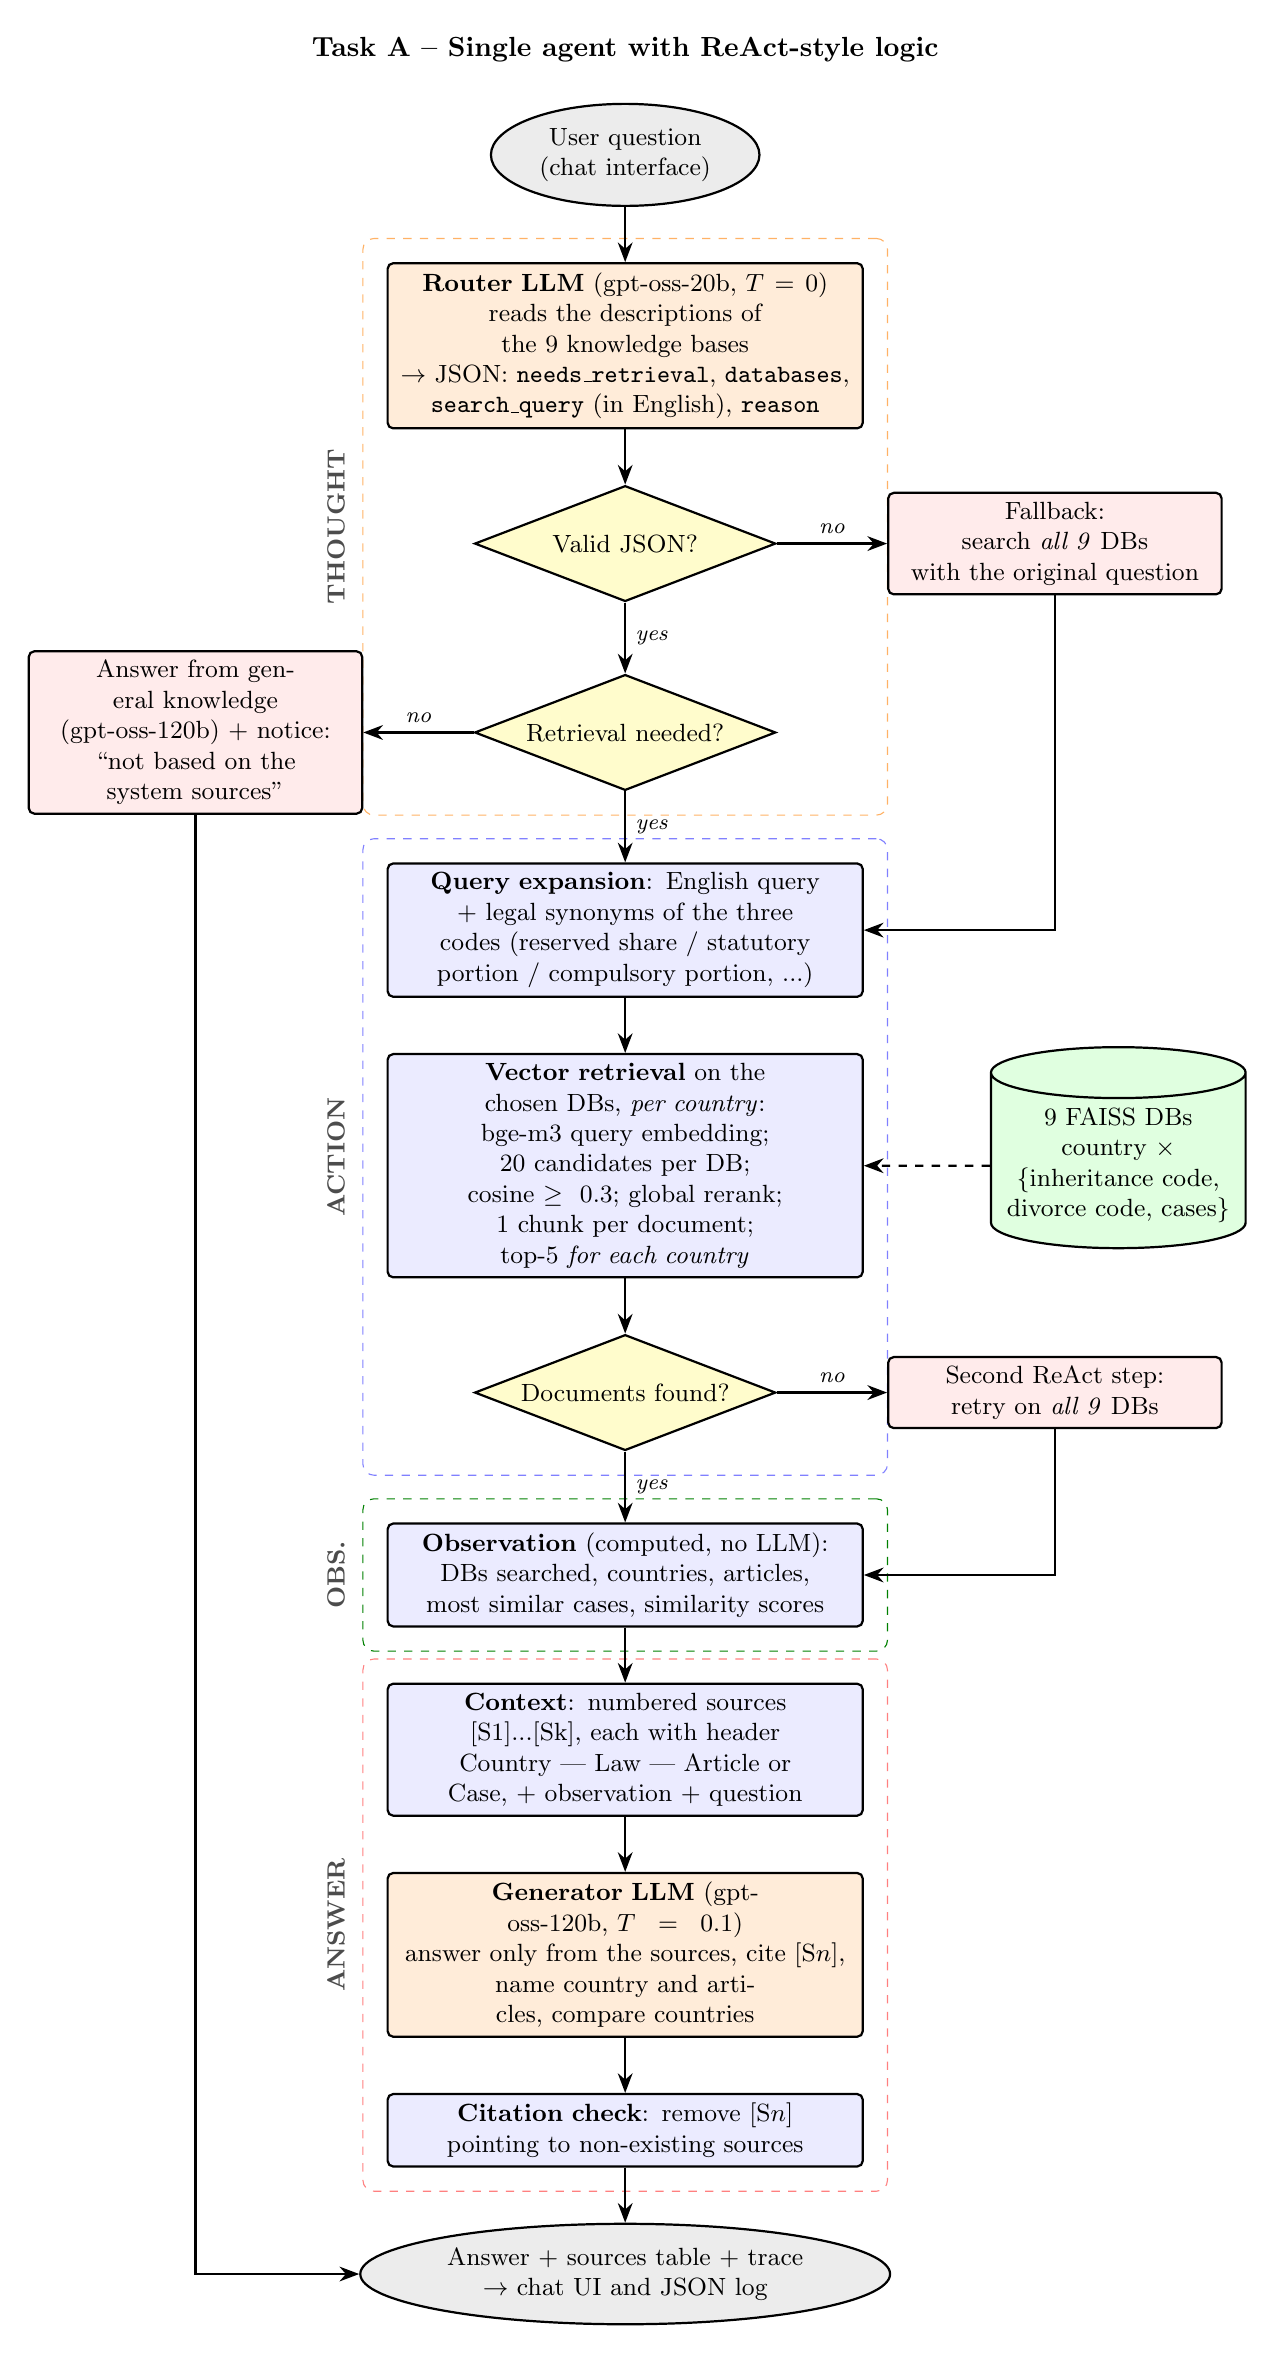
\begin{tikzpicture}[node distance=7mm]

% ---------------- main flow ----------------
\node[io] (q) {User question\\(chat interface)};

\node[llm, below=of q] (router) {\textbf{Router LLM} (gpt-oss-20b, $T=0$)\\
  reads the descriptions of the 9 knowledge bases\\
  $\rightarrow$ JSON: \texttt{needs\_retrieval}, \texttt{databases},\\
  \texttt{search\_query} (in English), \texttt{reason}};
\node[dec, below=of router] (json) {Valid JSON?};
\node[dec, below=9mm of json] (need) {Retrieval needed?};

\node[proc, below=9mm of need] (expand) {\textbf{Query expansion}: English query + legal synonyms
  of the three codes (reserved share / statutory portion / compulsory portion, ...)};
\node[proc, below=of expand] (search) {\textbf{Vector retrieval} on the chosen DBs, \emph{per country}:\\
  bge-m3 query embedding; 20 candidates per DB;\\
  cosine $\geq 0.3$; global rerank; 1 chunk per document;\\
  top-5 \emph{for each country}};
\node[dec, below=of search] (found) {Documents found?};
\node[proc, below=9mm of found] (obs) {\textbf{Observation} (computed, no LLM):\\
  DBs searched, countries, articles,\\most similar cases, similarity scores};
\node[proc, below=of obs] (ctx) {\textbf{Context}: numbered sources [S1]...[Sk], each with header
  Country | Law | Article or Case, + observation + question};
\node[llm, below=of ctx] (gen) {\textbf{Generator LLM} (gpt-oss-120b, $T=0.1$)\\
  answer only from the sources, cite [S$n$],\\name country and articles, compare countries};
\node[proc, below=of gen] (check) {\textbf{Citation check}: remove [S$n$] pointing to non-existing sources};
\node[io, below=of check] (out) {Answer + sources table + trace\\$\rightarrow$ chat UI and JSON log};

% ---------------- side elements ----------------
\node[side, right=14mm of json] (all) {Fallback:\\search \emph{all 9} DBs\\with the original question};
\node[side, left=14mm of need] (nokb) {Answer from general knowledge\\(gpt-oss-120b) + notice:\\
  ``not based on the system sources''};
\node[side, right=14mm of found] (retry) {Second ReAct step:\\retry on \emph{all 9} DBs};
\node[db, right=16mm of search] (dbs) {9 FAISS DBs\\country $\times$\\\{inheritance code,\\divorce code, cases\}};

% ---------------- arrows ----------------
\draw[arr] (q) -- (router);
\draw[arr] (router) -- (json);
\draw[arr] (json) -- node[lbl, right] {yes} (need);
\draw[arr] (json) -- node[lbl, above] {no} (all);
\draw[arr] (all) |- (expand);
\draw[arr] (need) -- node[lbl, right] {yes} (expand);
\draw[arr] (need) -- node[lbl, above] {no} (nokb);
\draw[arr] (nokb) |- (out);
\draw[arr] (expand) -- (search);
\draw[arr, dashed] (dbs) -- (search);
\draw[arr] (search) -- (found);
\draw[arr] (found) -- node[lbl, right] {yes} (obs);
\draw[arr] (found) -- node[lbl, above] {no} (retry);
\draw[arr] (retry) |- (obs);
\draw[arr] (obs) -- (ctx);
\draw[arr] (ctx) -- (gen);
\draw[arr] (gen) -- (check);
\draw[arr] (check) -- (out);

% ---------------- ReAct phases ----------------
\begin{scope}[on background layer]
  \node[fit=(router)(json)(need), draw=orange!60, dashed, rounded corners, inner sep=3mm] (pT) {};
  \node[fit=(expand)(search)(found), draw=blue!50, dashed, rounded corners, inner sep=3mm] (pA) {};
  \node[fit=(obs), draw=green!50!black, dashed, rounded corners, inner sep=3mm] (pO) {};
  \node[fit=(ctx)(gen)(check), draw=red!50, dashed, rounded corners, inner sep=3mm] (pAns) {};
\end{scope}
\node[phase] at ($(pT.west)+(-1mm,0)$) {THOUGHT};
\node[phase] at ($(pA.west)+(-1mm,0)$) {ACTION};
\node[phase] at ($(pO.west)+(-1mm,0)$) {OBS.};
\node[phase] at ($(pAns.west)+(-1mm,0)$) {ANSWER};

\node[font=\bfseries, above=4mm of q] {Task A -- Single agent with ReAct-style logic};
\end{tikzpicture}
\end{document}
